\begin{figure}
	\center
	\begin{minipage}{0.27\linewidth}
		\center \scriptsize
		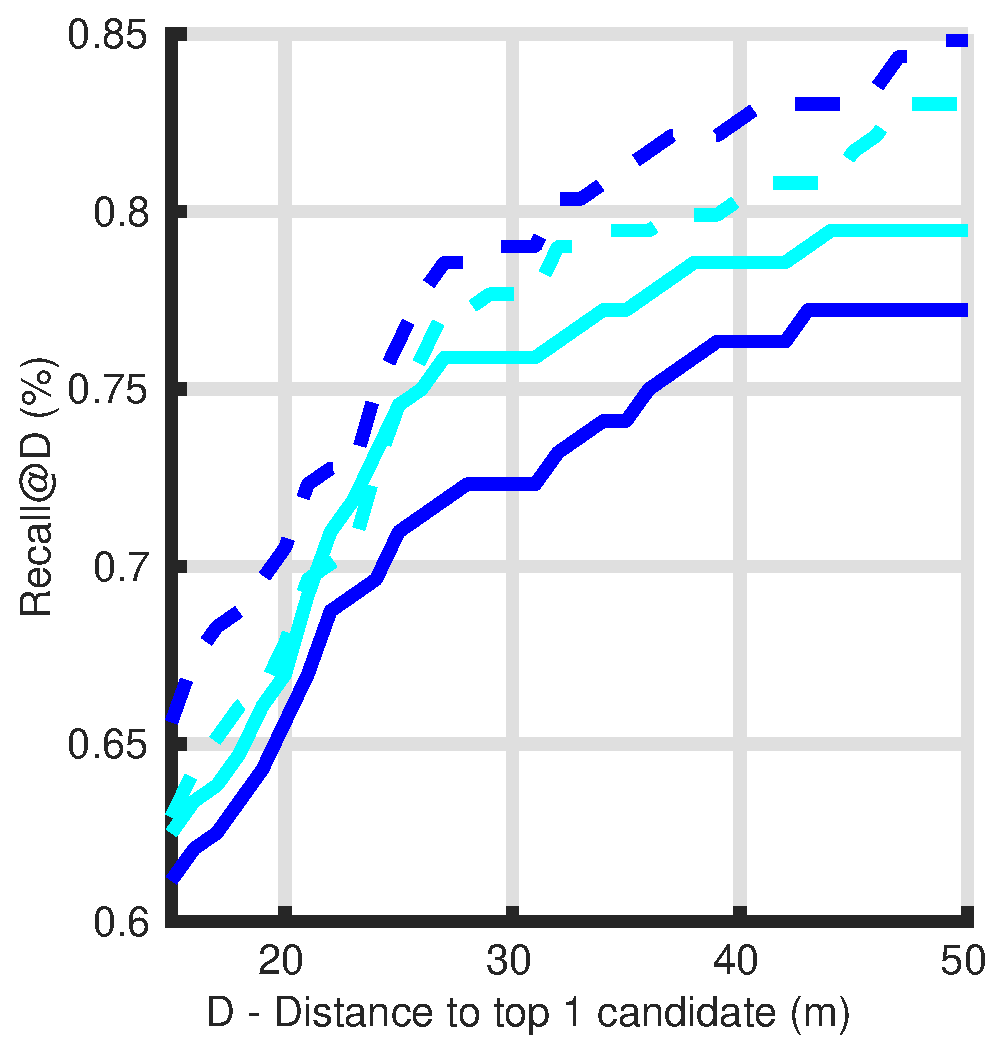
\includegraphics[width=\linewidth]{plot/night_ft/Results_lt_queries/distance}	
		
		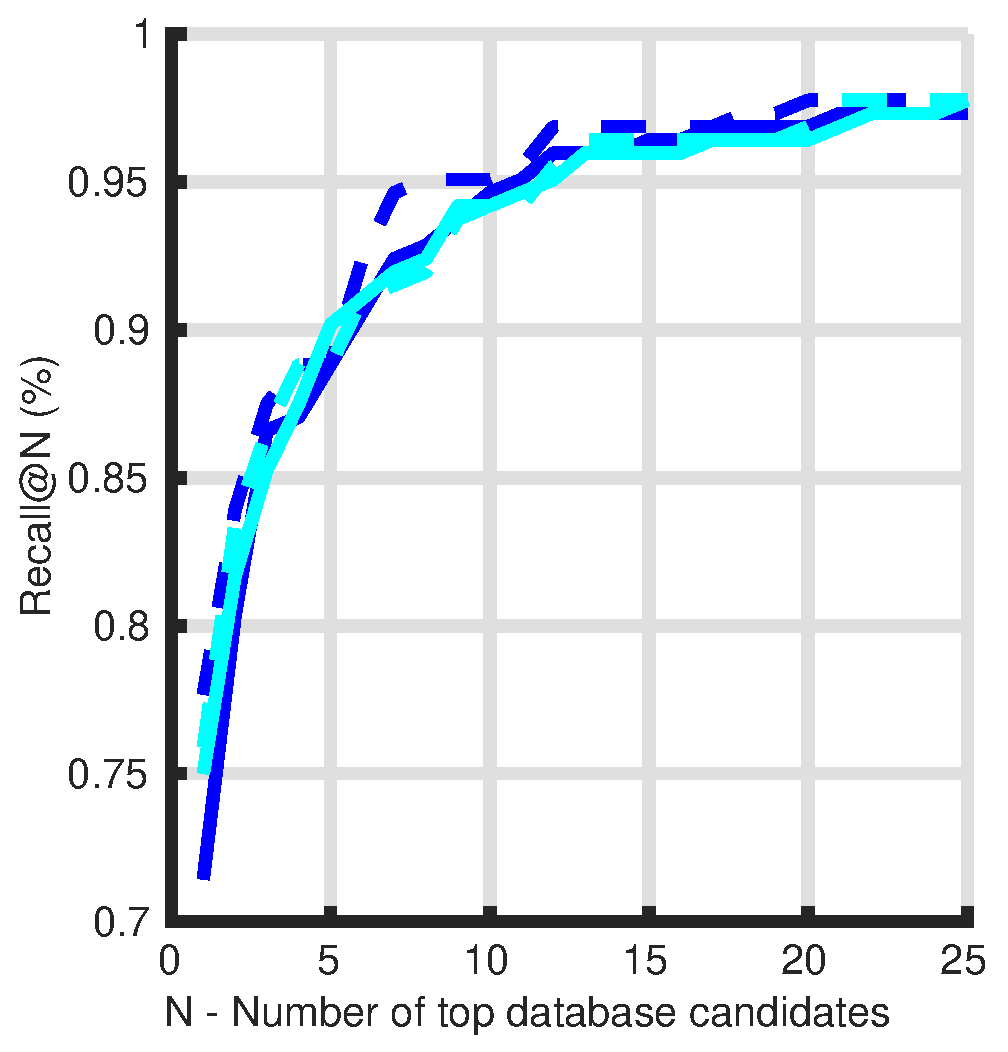
\includegraphics[width=\linewidth]{plot/night_ft/Results_lt_queries/recall}
		
		a) Oxford -- LT
	\end{minipage}
	\begin{minipage}{0.27\linewidth}
		\center \scriptsize
		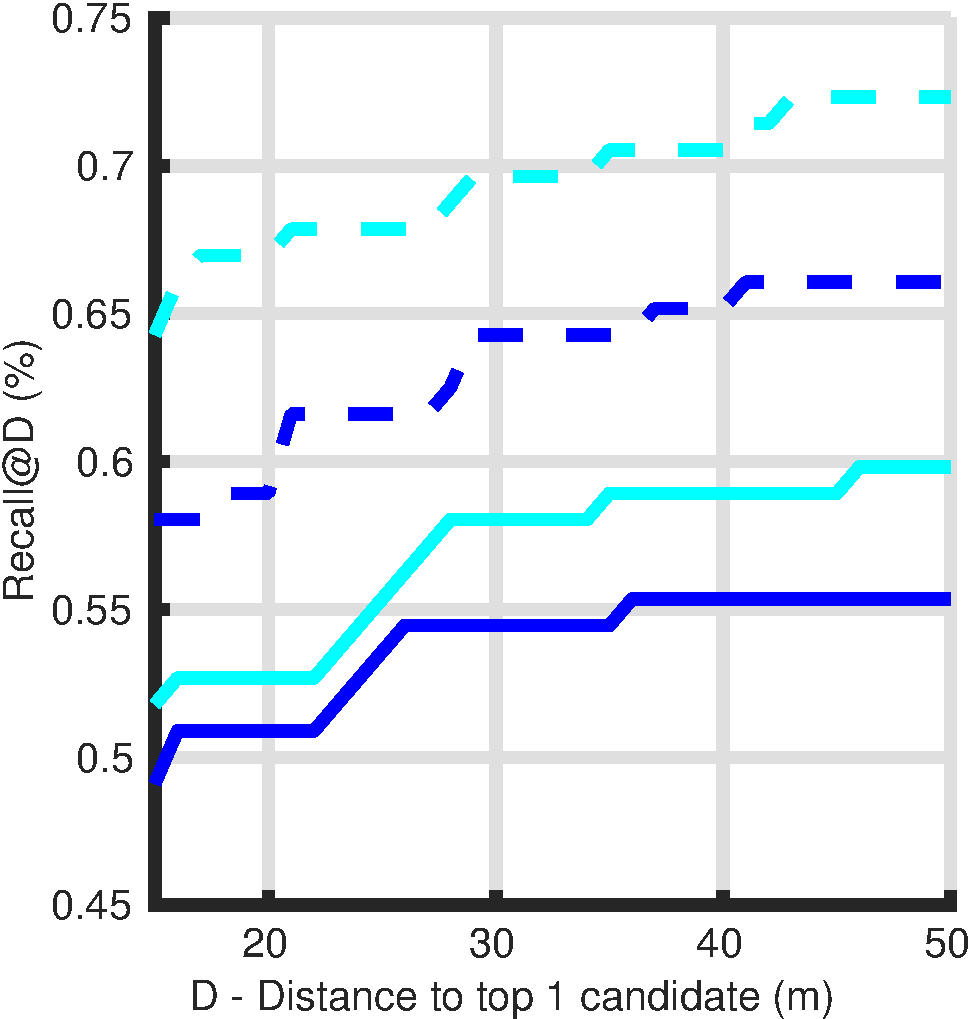
\includegraphics[width=\linewidth]{plot/night_ft/Results_snow_queries/distance}	
		
		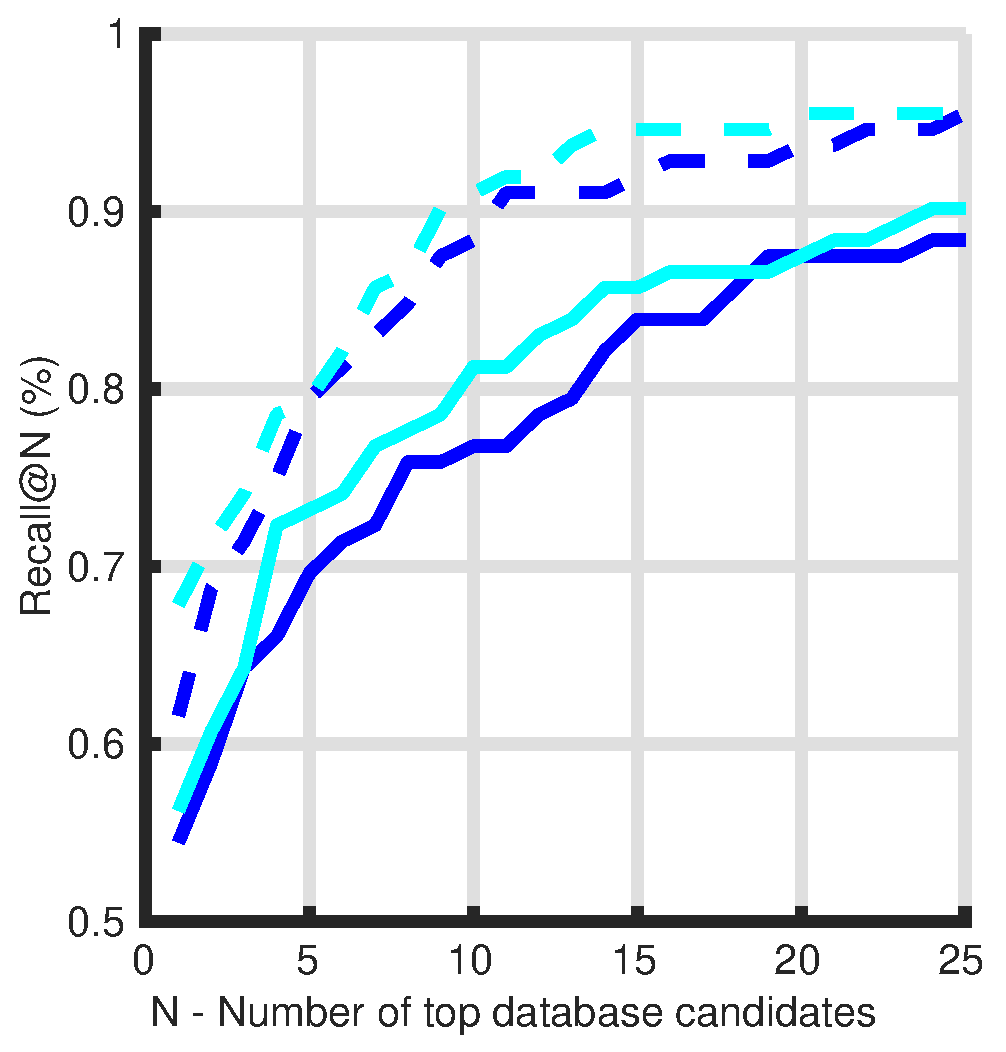
\includegraphics[width=\linewidth]{plot/night_ft/Results_snow_queries/recall}
				
		b) Oxford -- Snow
	\end{minipage}
	\begin{minipage}{0.27\linewidth}
		\center \scriptsize
		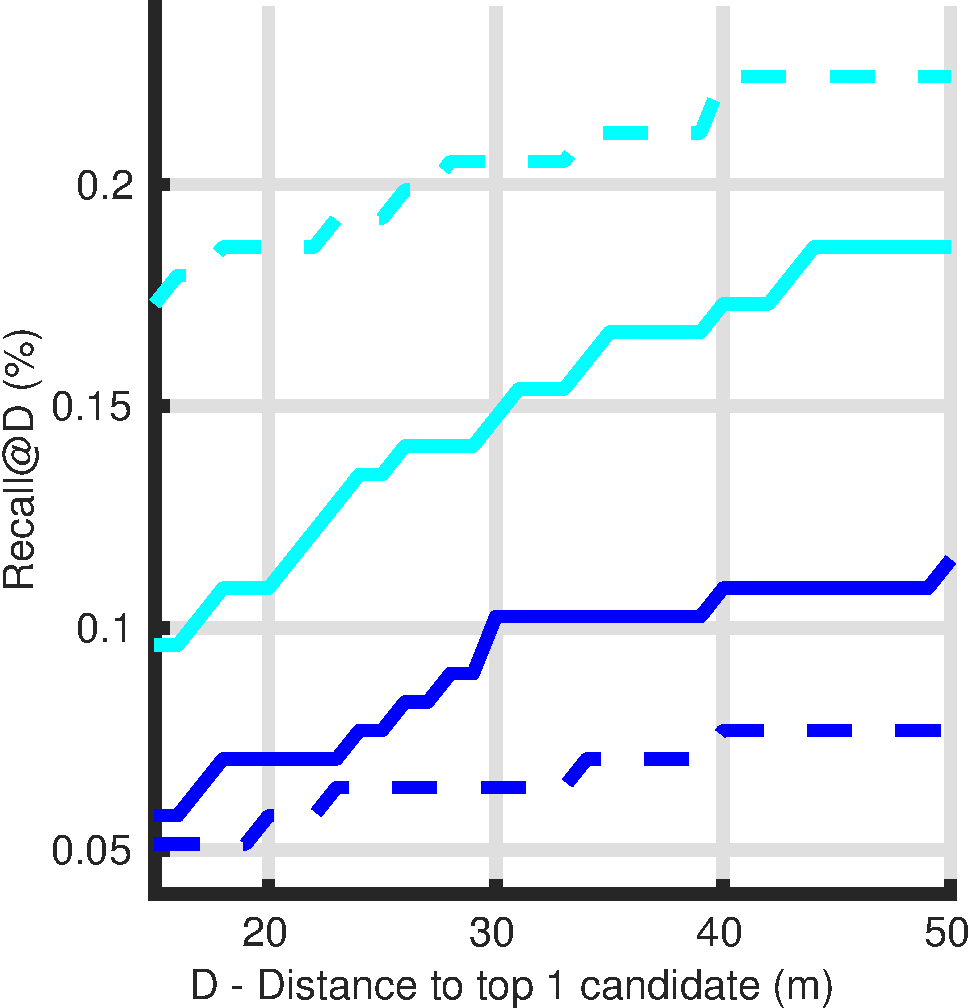
\includegraphics[width=\linewidth]{plot/night_ft/Results_night_queries/distance}	
		
		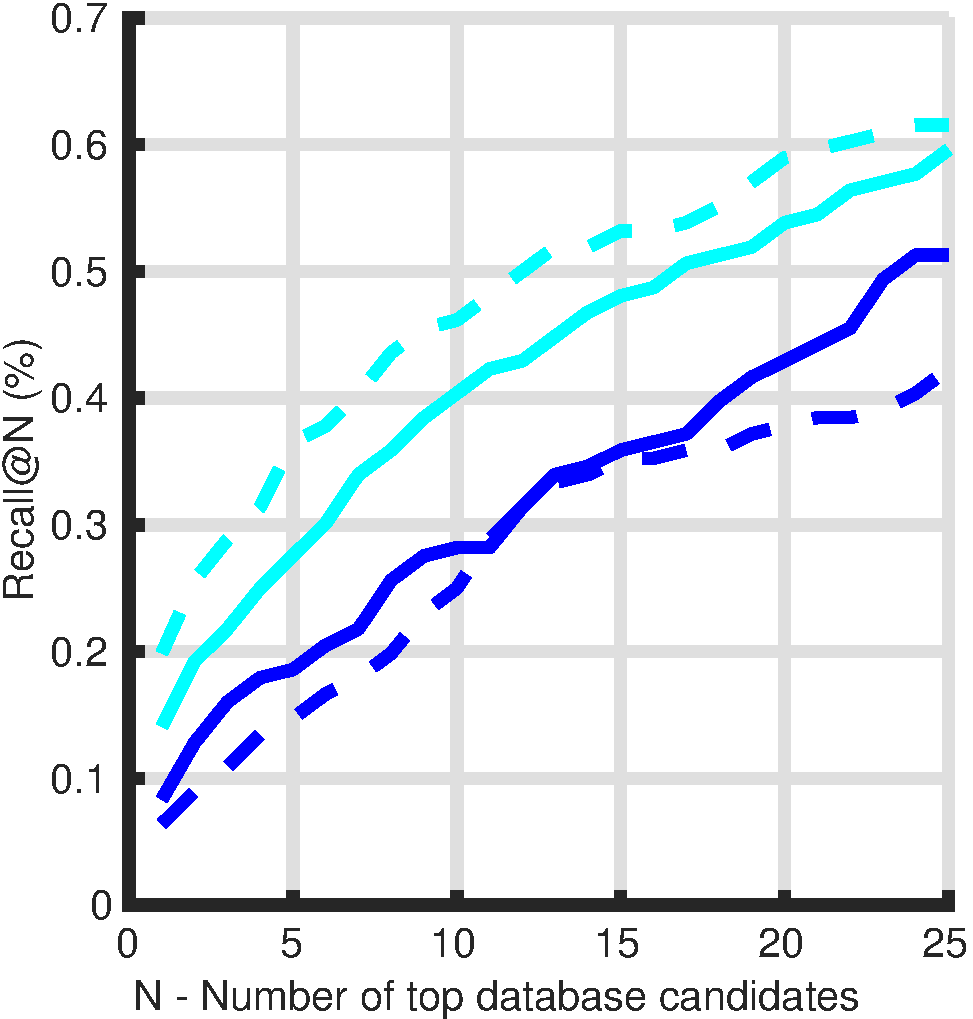
\includegraphics[width=\linewidth]{plot/night_ft/Results_night_queries/recall}
		
		c) Oxford -- Night
	\end{minipage}

	\vspace{5pt}	
	
	\begin{minipage}{0.27\linewidth}
		\center \scriptsize
		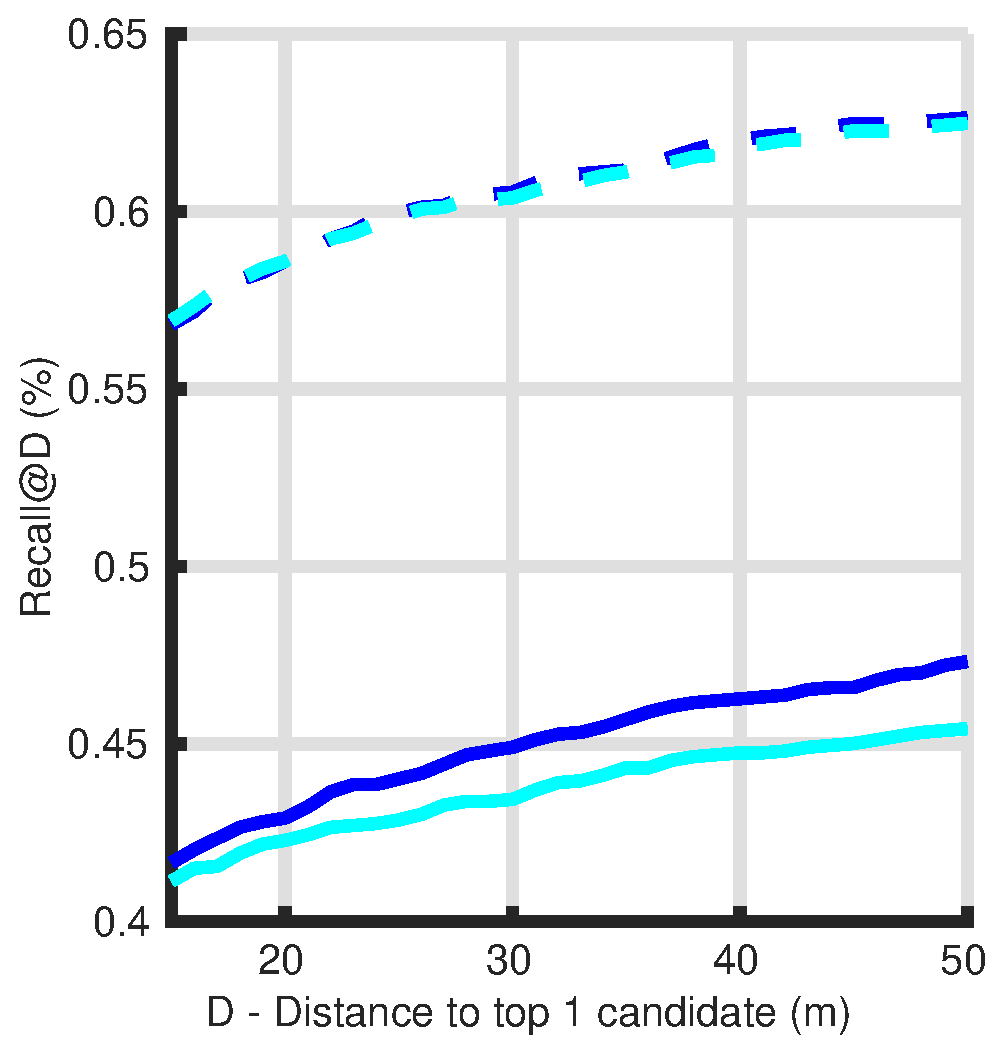
\includegraphics[width=\linewidth]{plot/night_ft/Results_cmu_lt/distance}	
		
		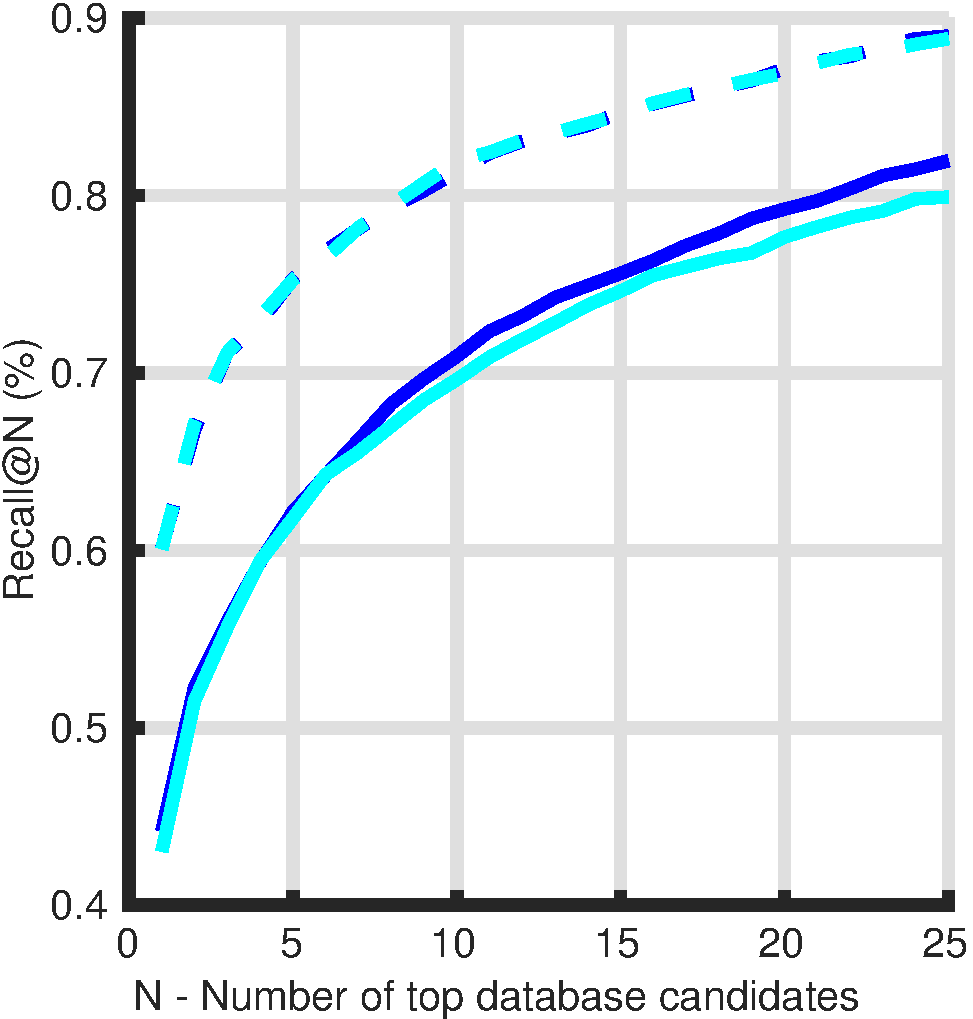
\includegraphics[width=\linewidth]{plot/night_ft/Results_cmu_lt/recall}
		
		d) CMU -- LT
	\end{minipage}
	\begin{minipage}{0.27\linewidth}
		\center \scriptsize
		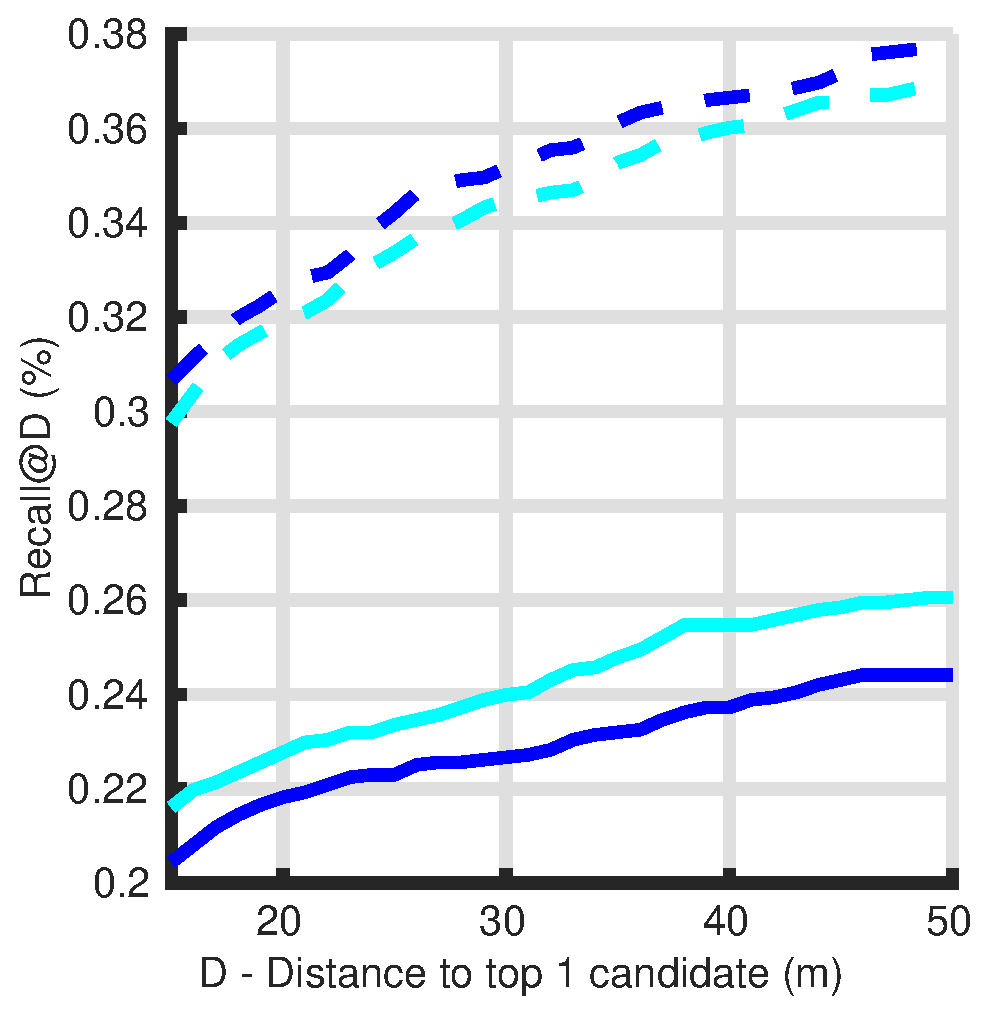
\includegraphics[width=\linewidth]{plot/night_ft/Results_cmu_snow/distance}	
		
		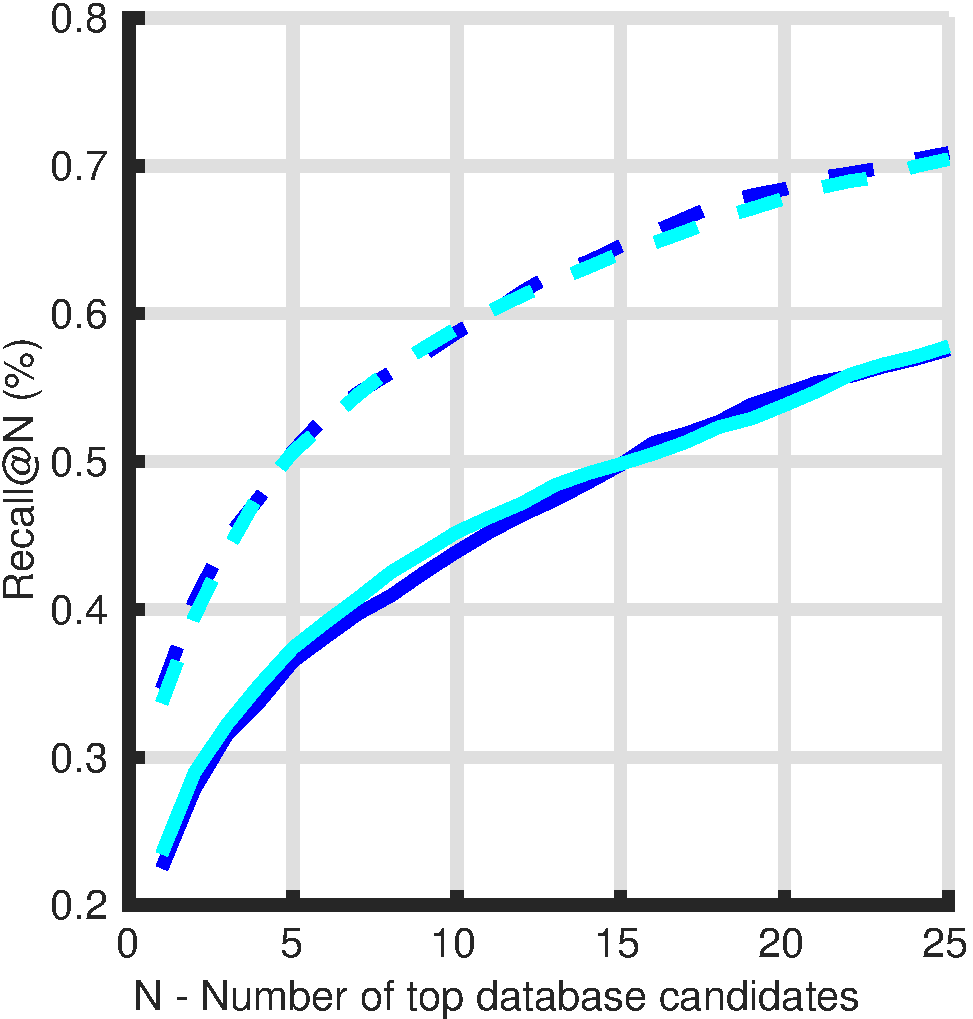
\includegraphics[width=\linewidth]{plot/night_ft/Results_cmu_snow/recall}
		
		e) CMU -- Snow
	\end{minipage}
	\begin{minipage}{0.27\linewidth}
		\center \scriptsize
		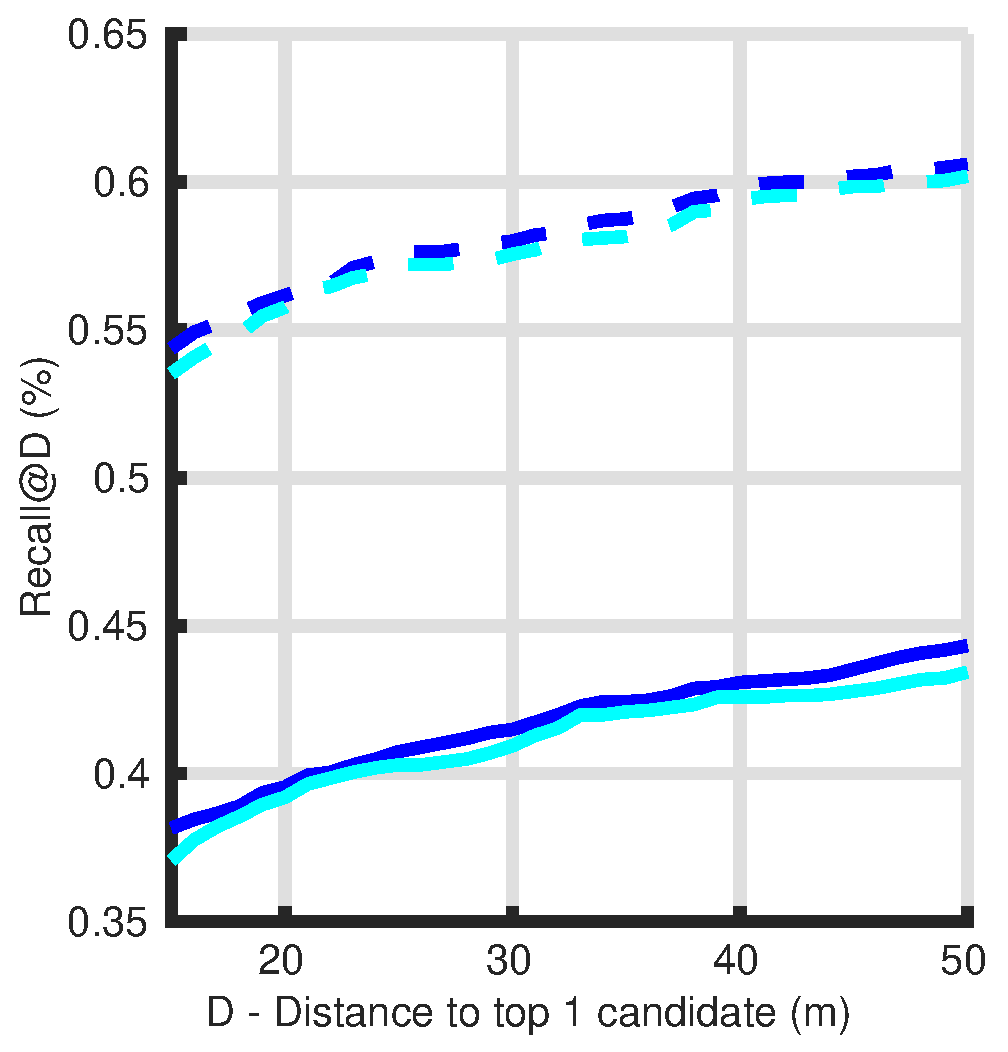
\includegraphics[width=\linewidth]{plot/night_ft/Results_cmu_autumn/distance}	
		
		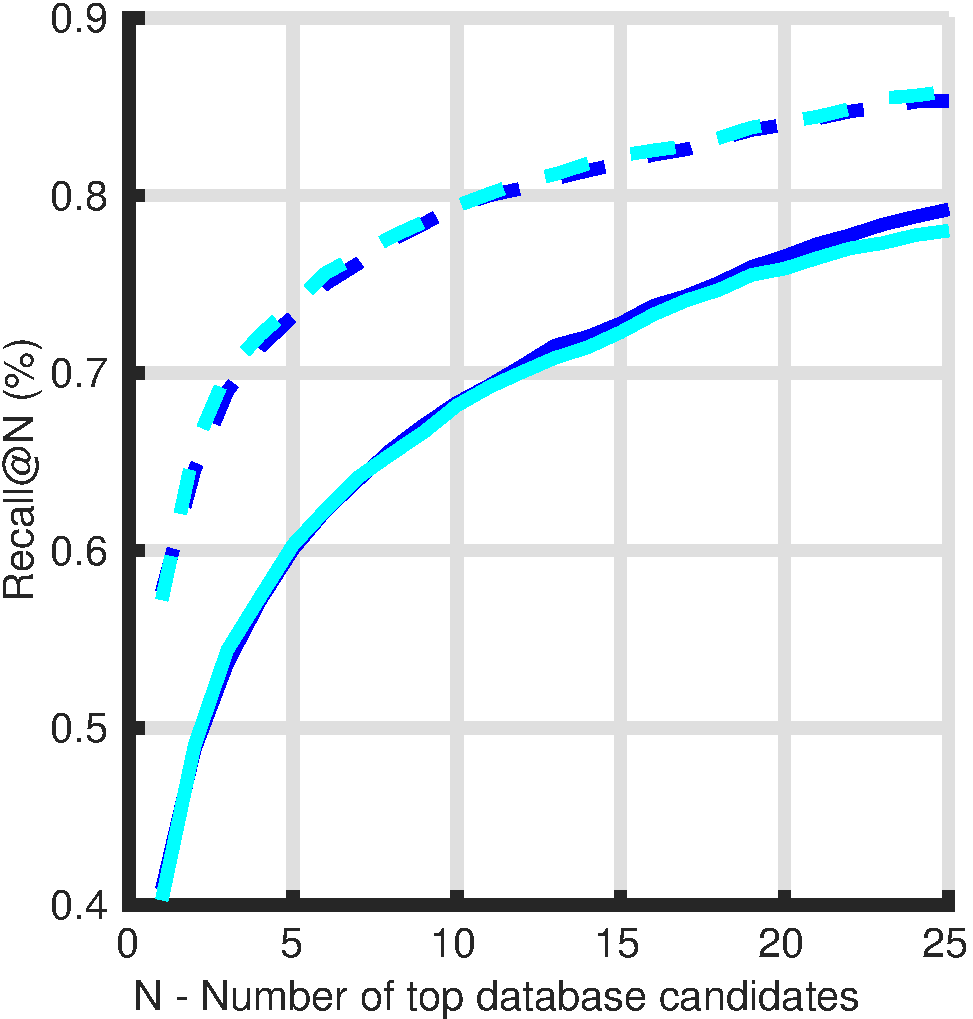
\includegraphics[width=\linewidth]{plot/night_ft/Results_cmu_autumn/recall}
		
		f) CMU -- Autumn
	\end{minipage}
	
	\vspace{0.2cm}
		
	\begin{scriptsize}
	\begin{tabular}{c l c l}
		\textcolor{blue}{\textbf{--}} & Alexnet RGB(D) & \textcolor{cyan}{\textbf{--}} & Alexnet RGB(D) fine tuned \\
		\textcolor{blue}{\textbf{- -}} & Resnet RGB(D) & \textcolor{cyan}{\textbf{- -}} & Resnet RGB(D) fine tuned \\
	\end{tabular}		
	\end{scriptsize}
	
	\caption[Results after fine tuning]{\label{fig:ft_night} \textbf{Results after fine tuning:} we are able to drastically improve localization performance for the Oxford -- Night challenging scenario (c) by only fine tuning the decoder part of our network with weakly annotated data. Curves best viewed in color.}
\end{figure}
